\section{Результаты} \label{section:results}

В целом, алгоритм показал себя хорошо: на некоторах типов зубов показатели COV метрики достигали значений 0.9. Что при столь малом размере выборки является очень хорошим результатом. Для избеганий зависимости от разбиений выборки на тестовую и обучающую части была использована кросс-валиадация, с коэффициентом разбиения 10.

\subsection{Программная реализаций}

Алгоритм был реализован на языке Python3 с использованием библиотек Numpy, Open3D и Sklearn. Для построения графиков использовалась библиотека matplotlib. В качестве среды разработки использовался Jupyter Notebook. \par
Для обучения на вход алгоритму подается обучающая выборка. Для генерации объектов алгоритму необходимо передать число используемых главных компонент и количество генерируемых данных. \par
Алгоритм обучения и генерации выборки размером в 150 элементов на компьютере MacBook Pro(2015) с процессором 2,7 GHz Intel Core i5 при размере обучающей выборки в 150 элементов работает меньше чем за секунду. Во многом, такая скорость была достигнута за счет использования KD-деревьев для расчета CD-расстояния (см. \ref{section:metrics-comparation}). \par
Тем не менее, расчет метрик для оценивания качества сгенерированных объектов занимает существенно большое количество времени. К примеру, вычисление COV и MMD метрик между двумя группами объектов в 150 и 15 элементов и при среднем количестве точек в объекте равном 2500 точек занимает 28 секунд. 


\subsection{Метрики}

Пример результата вычисления значения метрик предствлен на рис. \ref{fig:res_example}. По оси X распололжены значения количества используемых главных компонент, по оси Y представлены значения метрик. Метрики вычисляются для значений числа компонент от 1 до 15.

\begin{figure}[h]
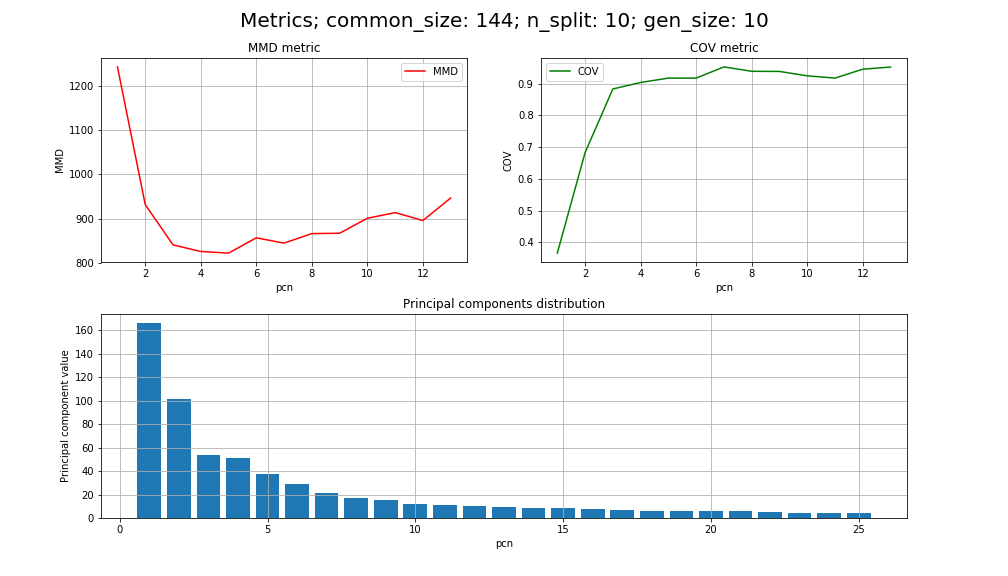
\includegraphics[width=1\linewidth]{images/res_example.png}
\caption{Пример значений метрик}
\label{fig:res_example}
\end{figure}

\subsection{Зависимость показателей метрик от коэффициента при $\sigma$}

Выбор коэффициента $c$ при $\sigma$ (см. \ref{section:algorithm:generation}) имеет большое влияние на качество работы алгоритма. На рисунках \ref{fig:c_diff_1}, \ref{fig:c_diff_2} показаны зависимость метрик от коэффициента $c$ для двух разных типов зубов и для трех значений $c$ равных $1.0; 2.0; 3.0$. Как видно из графиков наилучшие показатели метрик  достигаются при значениях $c = 3.0$. \par

Рисунок \ref{fig:c_diff_3} показывает значения метрик в зависимости от значений $c$ равных $1.0; 2.0; 3.0; 3.5; 4.0$. С одной стороны, наилучшие показтели COV метрики достигаются при значении $c = 4.0$, но при этом график MMD метрики становится нестабильным и при достижении своего локального минимума начинает расти вверх, что не так сильно выражено для графика при $c = 3.0$. График для $c = 3.5$ также не является стабильным. Более того, сравнение графиков MMD метрик при значениях $c$ равных $3.0; 3.5; 4.0$ показывают, что увеличение значения параметрка $c$ ухудшает показатели MMD метрики. \par
Золотой серединой является показатель $c = 3.0$: при нем наблюдается стабильность графика MMD и достижение им наименьшего значения, и высокие показатели COV метрики.

\begin{figure}[h]
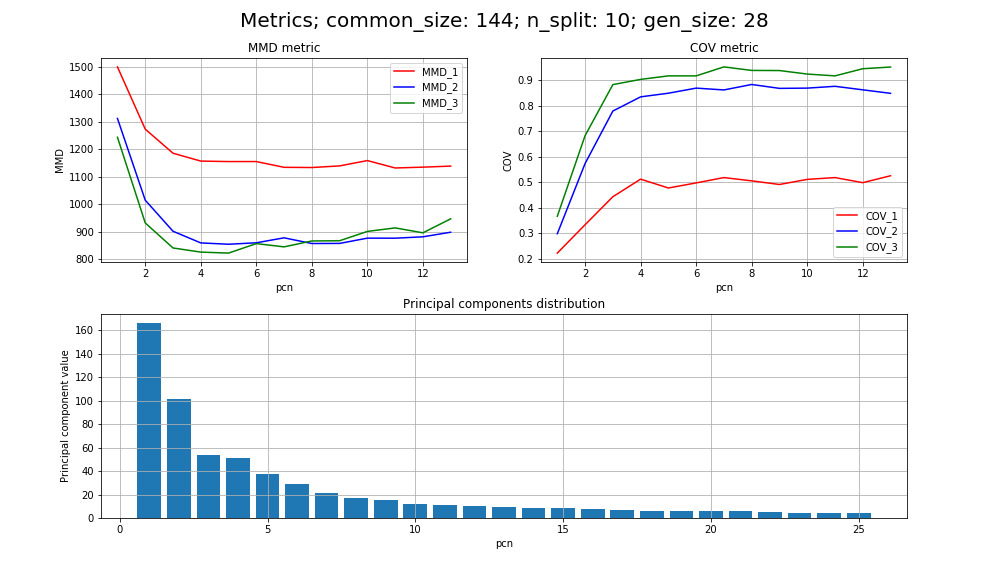
\includegraphics[width=1\linewidth]{images/c_diff_3_44.png}
\caption{Зависимость показателей метрик от коэффициента при $\sigma$. 
COV\_1, MMD\_1 для $c = 1.0$,  COV\_2, MMD\_2 для $c = 2.0$,  COV\_3, MMD\_3 для $c = 3.0$}
\label{fig:c_diff_1}
\end{figure}


\begin{figure}[h]
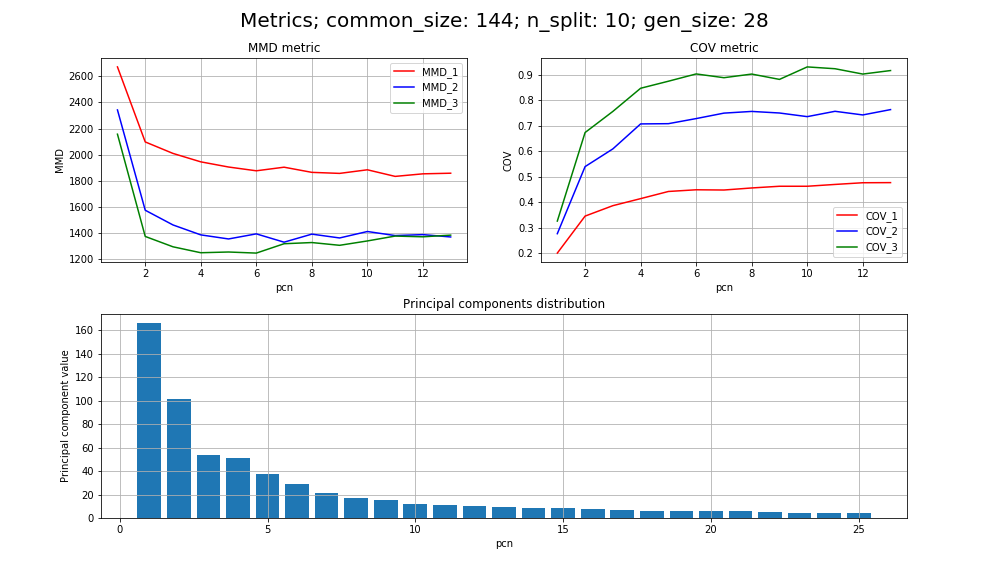
\includegraphics[width=1\linewidth]{images/c_diff_3_45.png}
\caption{Зависимость показателей метрик от коэффициента при $\sigma$.
COV\_1, MMD\_1 для $c = 1.0$,  COV\_2, MMD\_2 для $c = 2.0$,  COV\_3, MMD\_3 для $c = 3.0$}
\label{fig:c_diff_2}
\end{figure}

\begin{figure}[h]
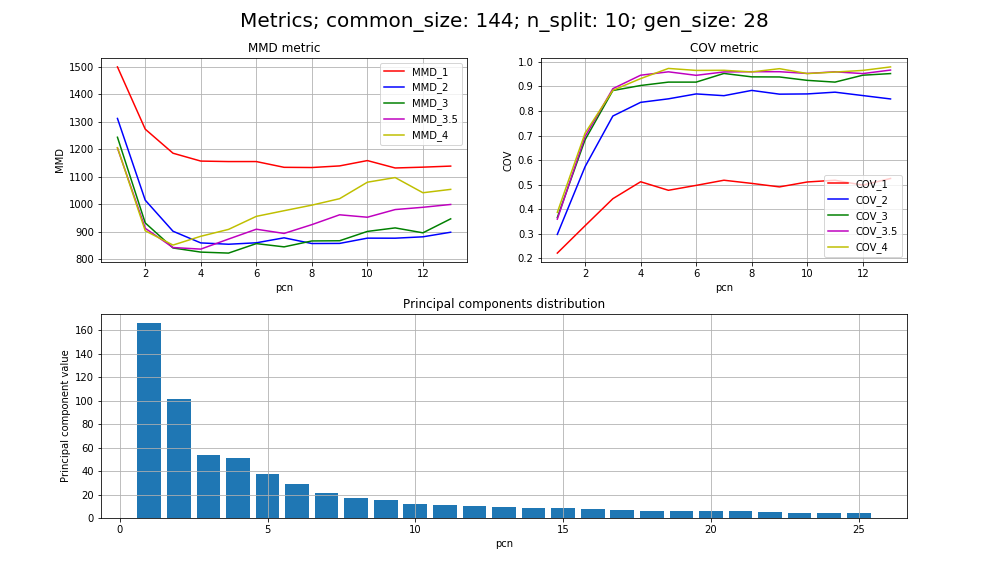
\includegraphics[width=1\linewidth]{images/c_diff_multiple.png}
\caption{Зависимость показателей метрик от коэффициента при $\sigma$.
COV\_1, MMD\_1 для $c = 1.0$,  COV\_2, MMD\_2 для $c = 2.0$,  COV\_3, MMD\_3 для $c = 3.0$,
COV\_3.5, MMD\_3.5 для $c = 3.5$,  COV\_4, MMD\_4 для $c = 4.0$}
\label{fig:c_diff_3}
\end{figure}

\subsection{Примеры данных}
На рисунках 16, 17 представлены результаты генерации новых зубов. Стоит отметить, что далеко не все сгенерированные данные удачны. Рис. 17 это хорошо показывает.

\begin{figure*}[ht!]
	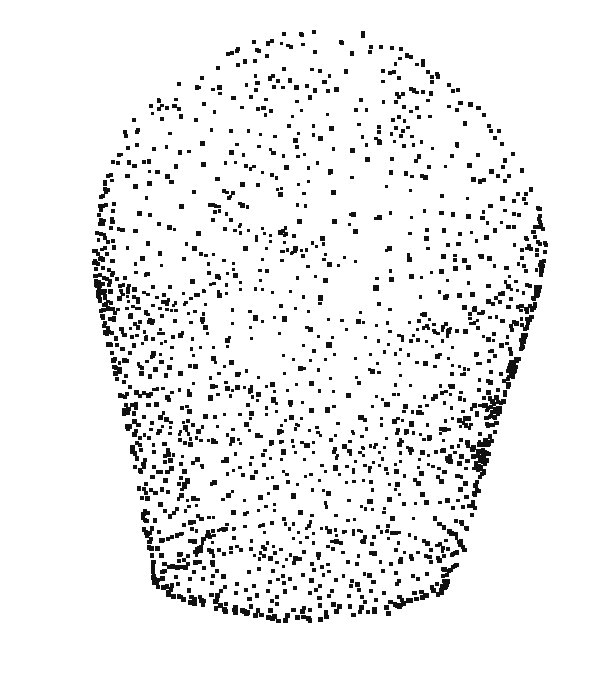
\includegraphics[width=.3\textwidth]{images/snapshot_44_1_002.png}\hfill
    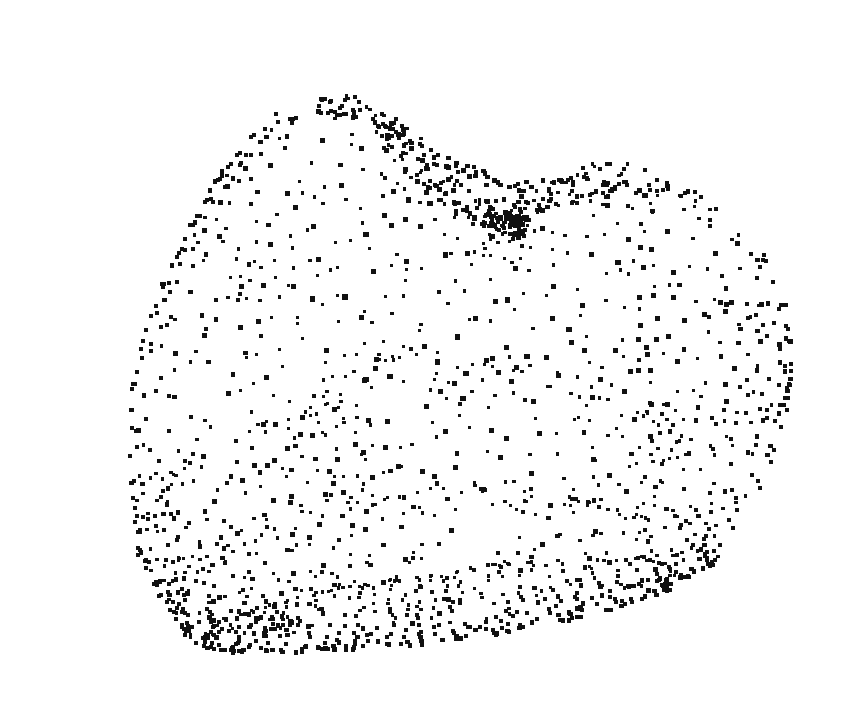
\includegraphics[width=.3\textwidth]{images/snapshot_ex01.png}\hfill
    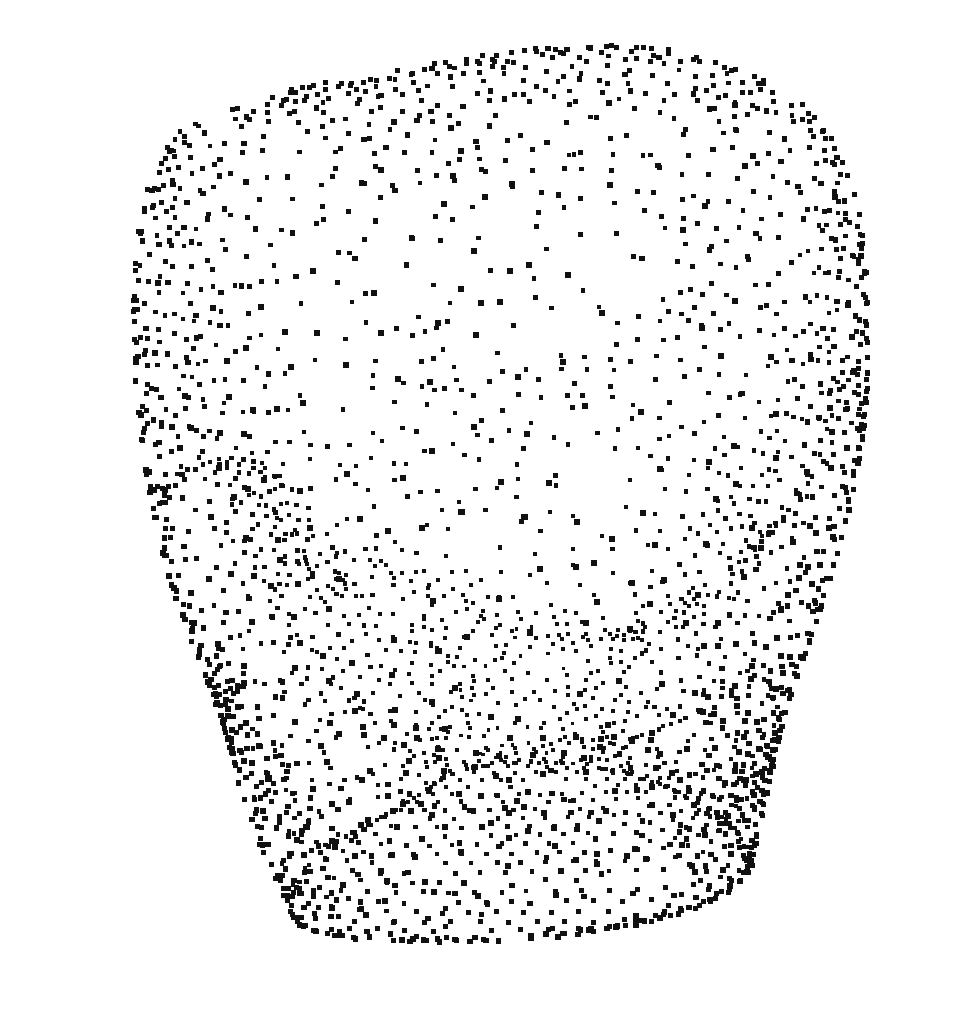
\includegraphics[width=.3\textwidth]{images/snapshot_mean00.png}
    \label{fig:gex1}
    \caption{Удачные примеры сгенерированных данных}
\end{figure*}
\begin{figure*}[ht!]
    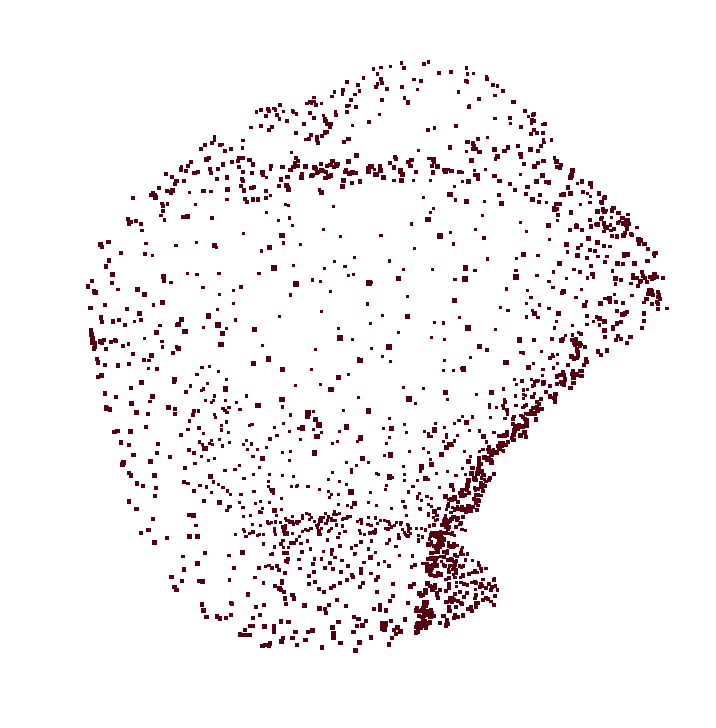
\includegraphics[width=.3\textwidth]{images/snapshot_ex_b02.png}\hfill
    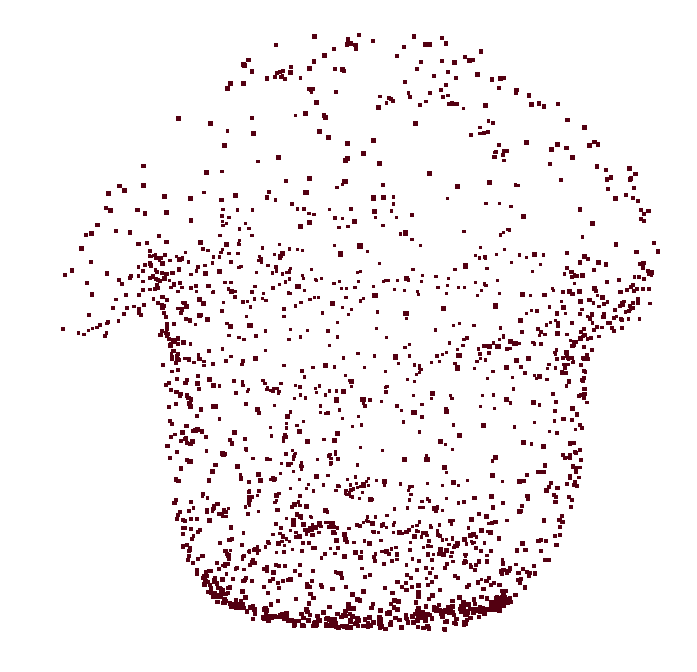
\includegraphics[width=.3\textwidth]{images/snapshot_ex_b04.png}\hfill
    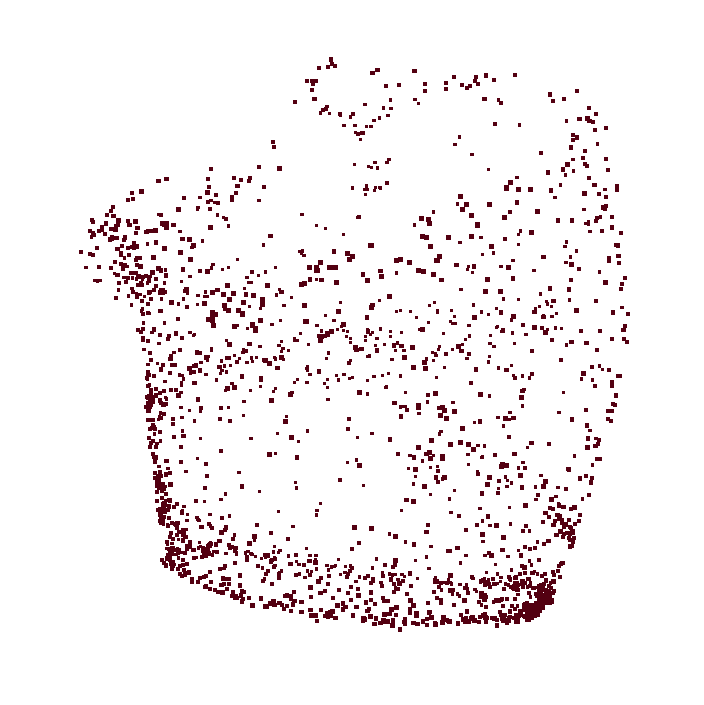
\includegraphics[width=.3\textwidth]{images/snapshot_ex_b06.png}
    \label{fig:gex2}
    \caption{Неудачные примеры cгенерированных данных}
\end{figure*}


\subsection{Исследования статистических свойств}
Для исследования статистических свойств были выполнены следующие эксперименты: взят вектор $\sigma = (\sigma_{1}, \ldots, \sigma_{K})$ и восстанавливать объекты со значениями в пространстве главных комопнент равными $-3.0 \cdot \sigma$, $-2.0 \cdot \sigma$, $-1.0 \cdot \sigma$, $0.0 \cdot \sigma$, $1.0 \cdot \sigma$, $2.0 \cdot \sigma$, $3.0 \cdot \sigma$. Результаты эксперимента показаны на рис. \ref{fig:c_l_1}, \ref{fig:c_l_2}, \ref{fig:c_l_3}, \ref{fig:c_l_4}.

На разные типы зубов изменение коэффициента $c$ влияет по-разному. Для первого премоляра (рис. \ref{fig:c_l_1}, \ref{fig:c_l_2}) увеличение коэффициента приводит к общему увеличению размера зуба, а для второго типа зубов (первых резцов, рис. \ref{fig:c_l_3}, \ref{fig:c_l_4}) отрицательные значения значения коэффициента уменьшают его ширину и увеличивают высоту. В свою очередь, положительные коэффициенты увеличивают ширину и уменьшают высоту.

Первый тип сгенерированных объектов представлен в увеличенном виде на рис. 22, второй тип - на рис. 23.

\begin{figure}[h]
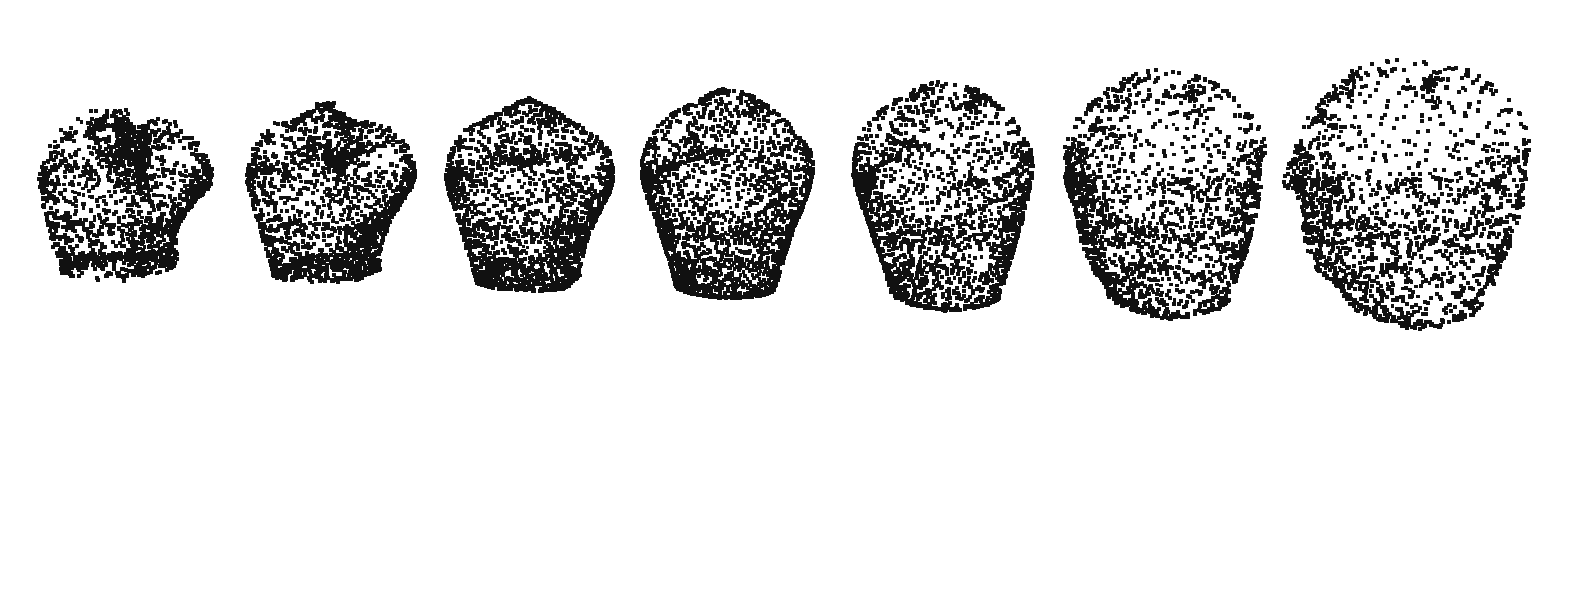
\includegraphics[width=1\linewidth]{images/snapshot_gen_44_var00.png}
\caption{Зависимость объектов от исходных значений равных $c \cdot \sigma$, $c$ увеличивается слева направо от $-3.0$ до $3.0$ с шагом $1.0$.}
\label{fig:c_l_1}
\end{figure}

\begin{figure}[h]
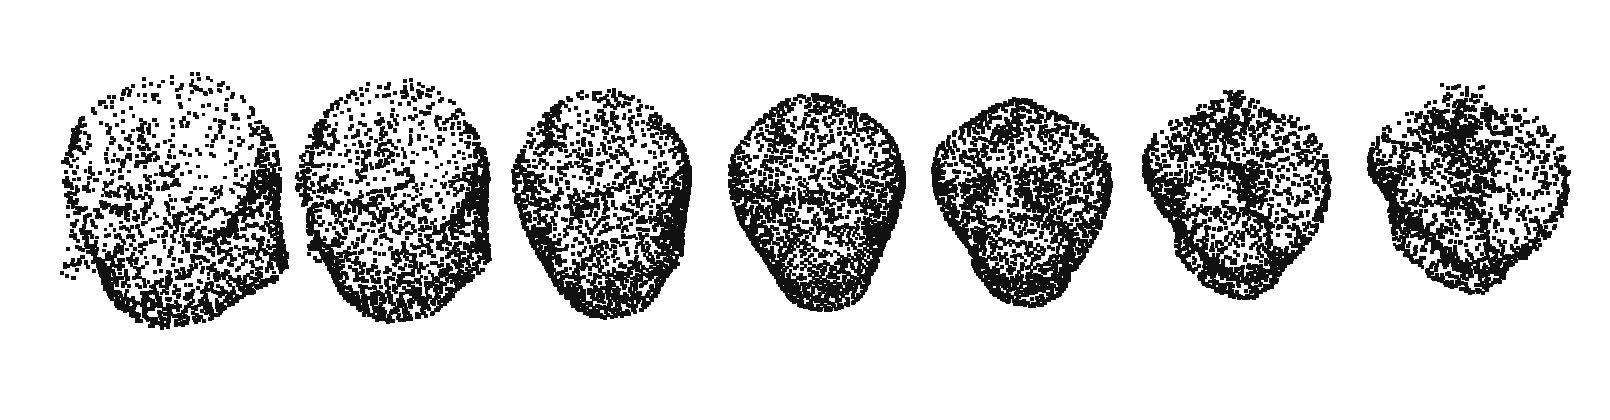
\includegraphics[width=1\linewidth]{images/snapshot_gen_44_var01.png}
\caption{Вид сзади. $c$ уменьшается слева направо от $3.0$ до $-3.0$ с шагом $1.0$.}
\label{fig:c_l_2}
\end{figure}


\begin{figure}[h]
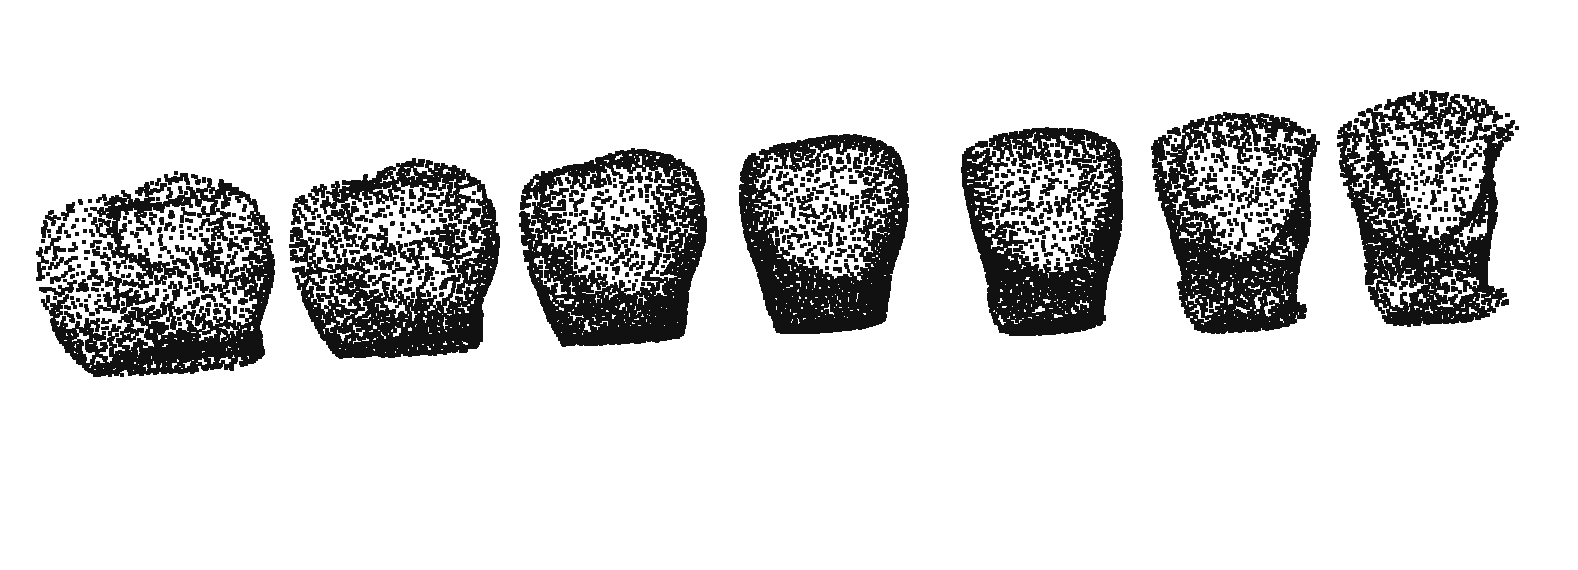
\includegraphics[width=1\linewidth]{images/snapshot_gen_var00.png}
\caption{Зависимость объектов от исходных значений равных $c \cdot \sigma$, $c$ увеличивается слева направо от $-3.0$ до $3.0$ с шагом $1.0$.}
\label{fig:c_l_3}
\end{figure}

\begin{figure}[h]
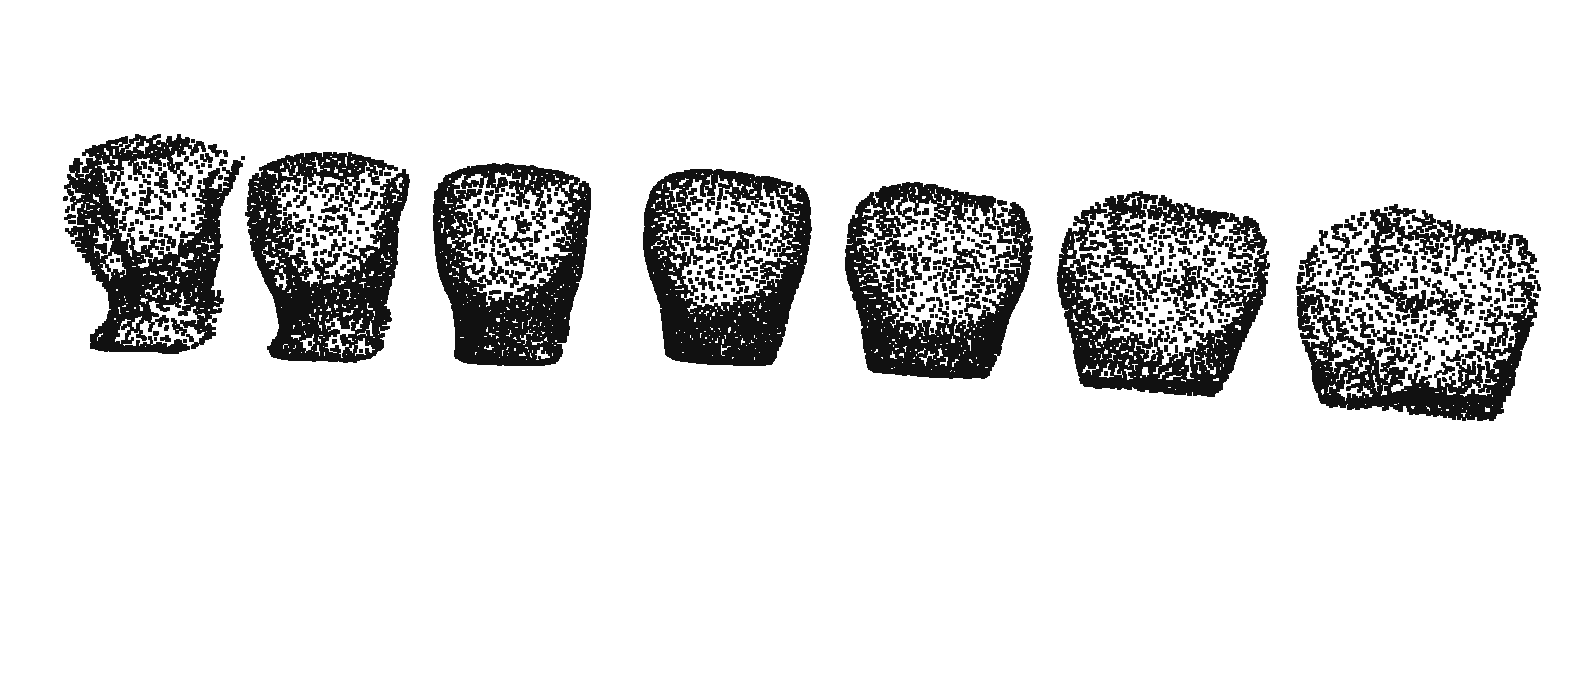
\includegraphics[width=1\linewidth]{images/snapshot_gen_var02.png}
\caption{Вид сзади. $c$ уменьшается слева направо от $3.0$ до $-3.0$ с шагом $1.0$.}
\label{fig:c_l_4}
\end{figure}


\begin{figure*}[ht!]
    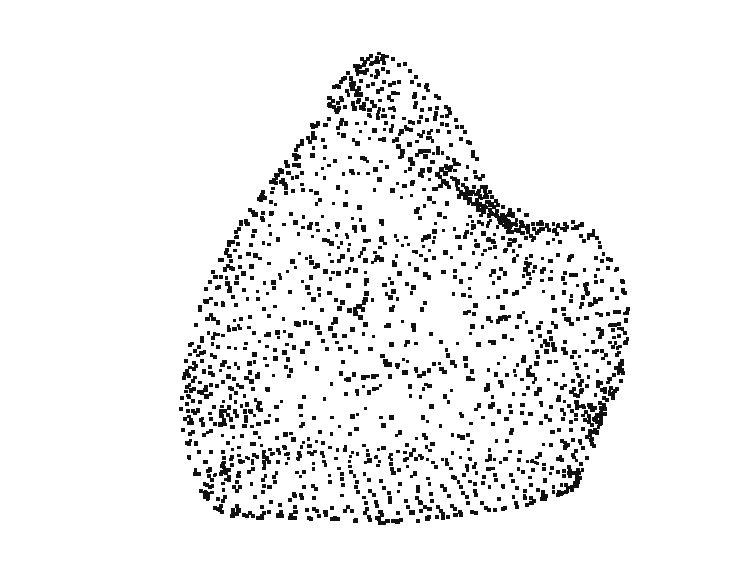
\includegraphics[width=.3\textwidth]{images/snapshot_44_-1_005.png}\hfill
    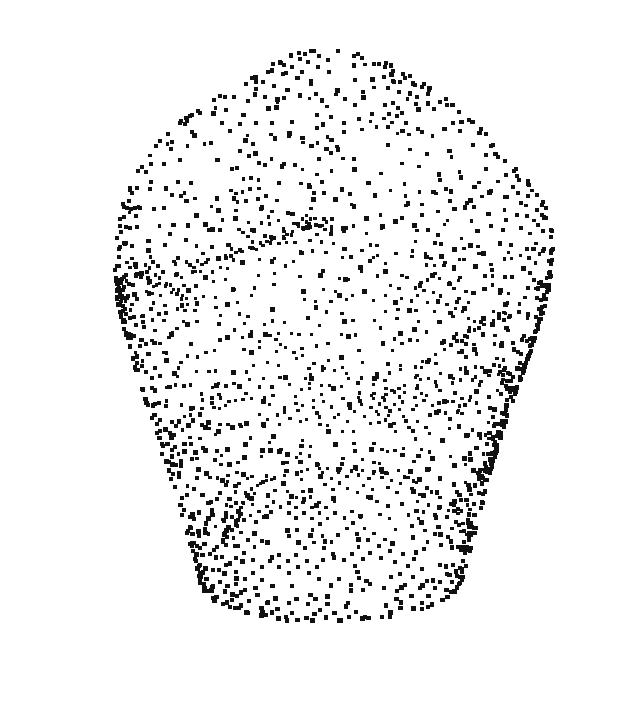
\includegraphics[width=.3\textwidth]{images/snapshot_44_mean00.png}\hfill
    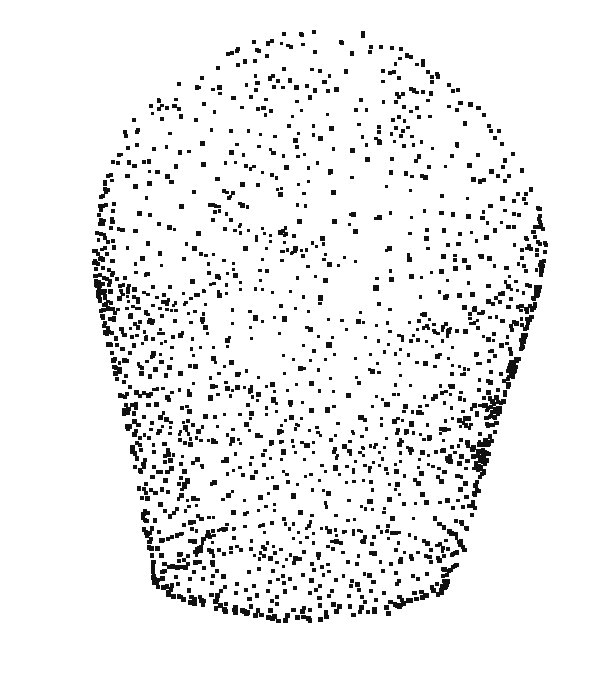
\includegraphics[width=.3\textwidth]{images/snapshot_44_1_002.png}
    \label{fig:gex3}
    \caption{Первый премоляр при значениях $c$ равных $-1.0; 0.0; 1.0$, слева направо}
\end{figure*}


\begin{figure*}[ht!]
    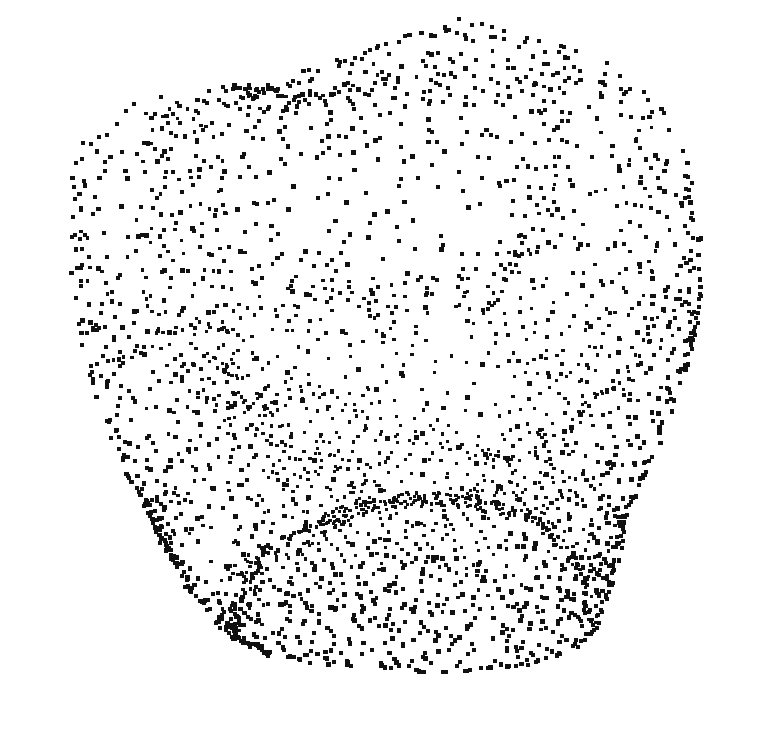
\includegraphics[width=.3\textwidth]{images/snapshot_11_-201.png}\hfill
    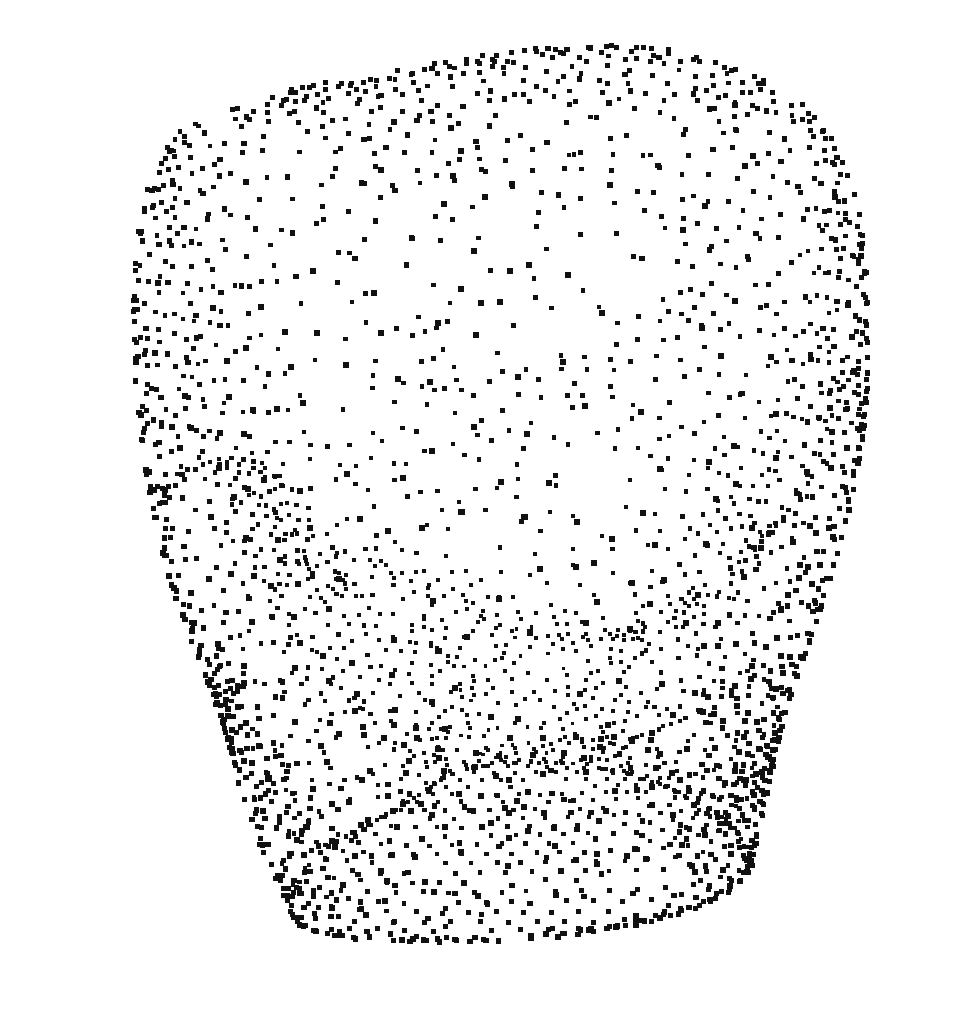
\includegraphics[width=.3\textwidth]{images/snapshot_mean00.png}\hfill
    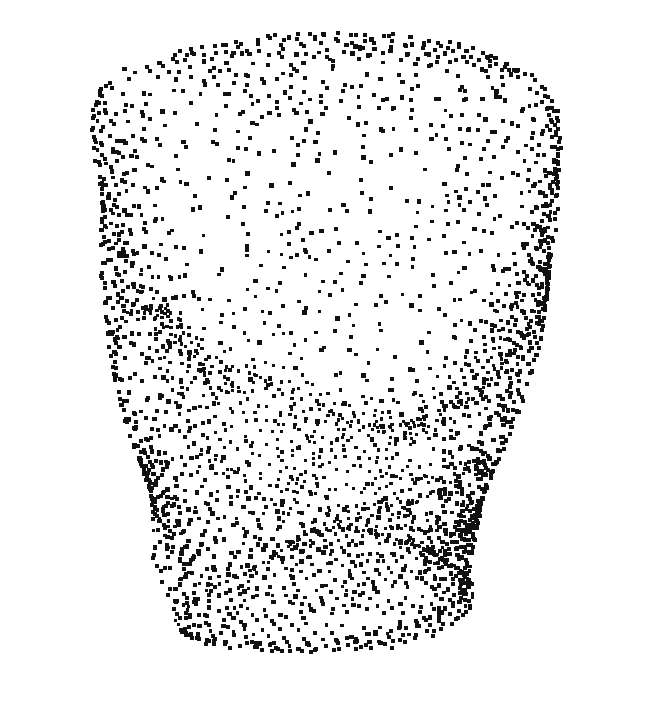
\includegraphics[width=.3\textwidth]{images/snapshot_1100.png}
    \label{fig:gex4}
    \caption{Первый резец при значениях $c$ равных $-2.0; 0.0; 1.0$, слева направо}
\end{figure*}

